\documentclass[a4j]{ujarticle}
\usepackage[dvipdfmx]{graphicx}
\usepackage{url}
\usepackage{bbding}
\usepackage{lscape}
\usepackage[subrefformat=parens]{subcaption}
\usepackage{bm}
\usepackage{amsmath}
\usepackage{ascmac}
\usepackage{comment}
\usepackage{ascmac}
% \usepackage{fancybx}
% \usepackage{minipage}

\title{補足資料}
\author{安達智哉\\to-adachi@ist.osaka-u.ac.jp}
\date{2019年12月19日}

\begin{document}
\maketitle





\begin{figure}[htbp]
 \centering
 \begin{subfigure}{0.49\hsize}
   \centering
   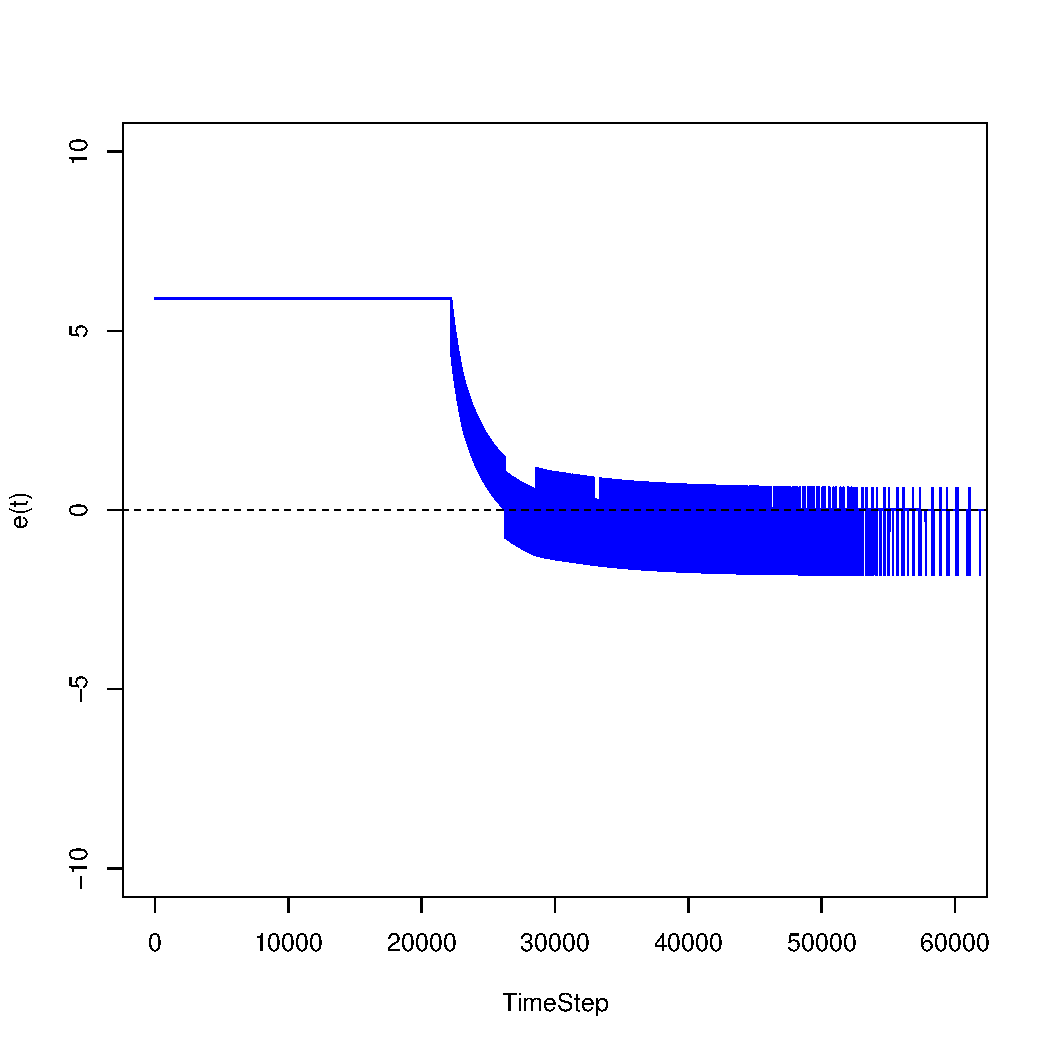
\includegraphics[width=1.0\hsize]{scenario_5_e_86400_345600_1_0_0_0_ideal.pdf}
   \subcaption{$e(t)$の変化}
   \label{subfig:scenario_5_e_86400_345600_0-318_1_0_0_0_ideal}
 \end{subfigure}
 \begin{subfigure}{0.49\hsize}
   \centering
   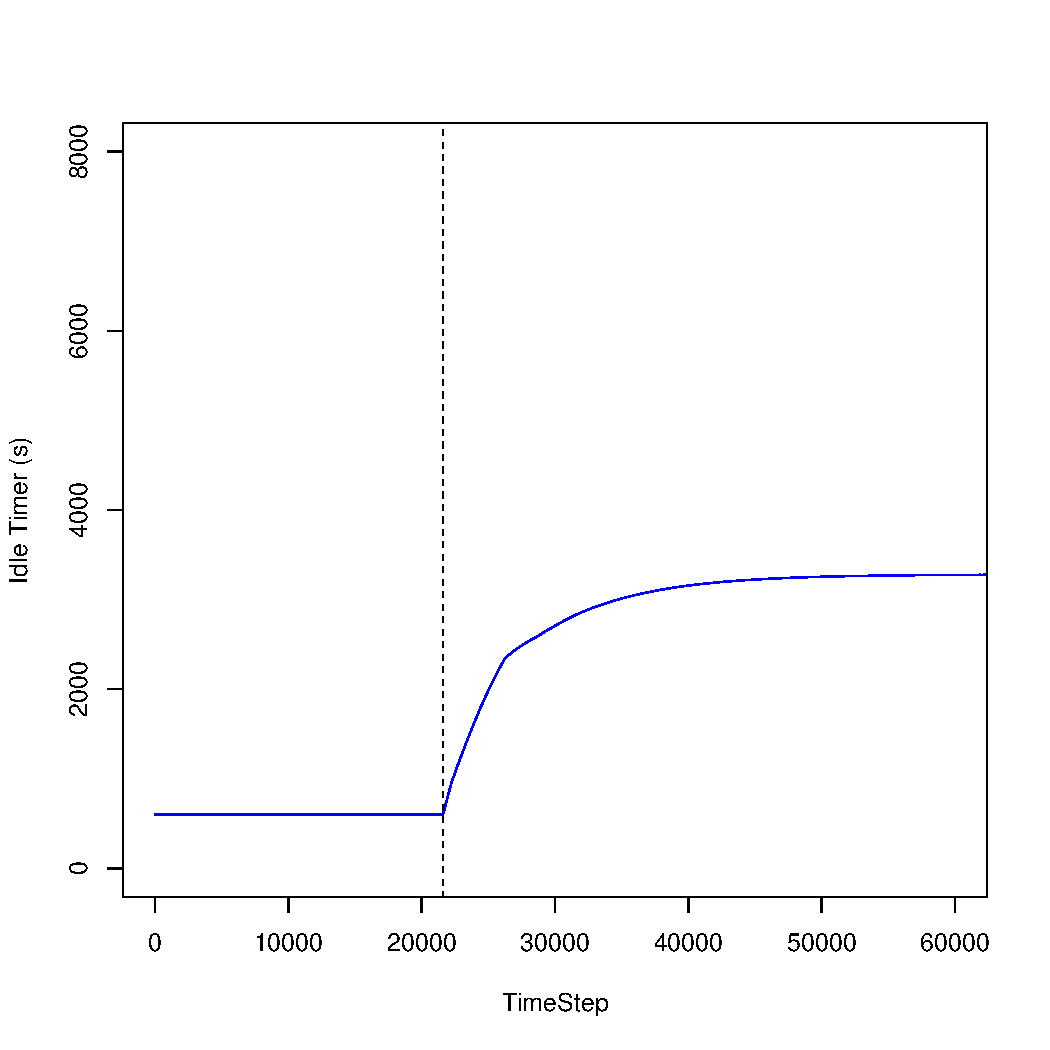
\includegraphics[width=1.0\hsize]{scenario_5_idleTimer_86400_345600_1_0_0_0_ideal.pdf}
   \subcaption{IdleTimerの変化}
   \label{subfig:scenario_5_idleTimer_86400_345600_1_0_0_0_ideal}
 \end{subfigure}
 \par\bigskip %改行
 \begin{subfigure}{0.49\hsize}
   \centering
   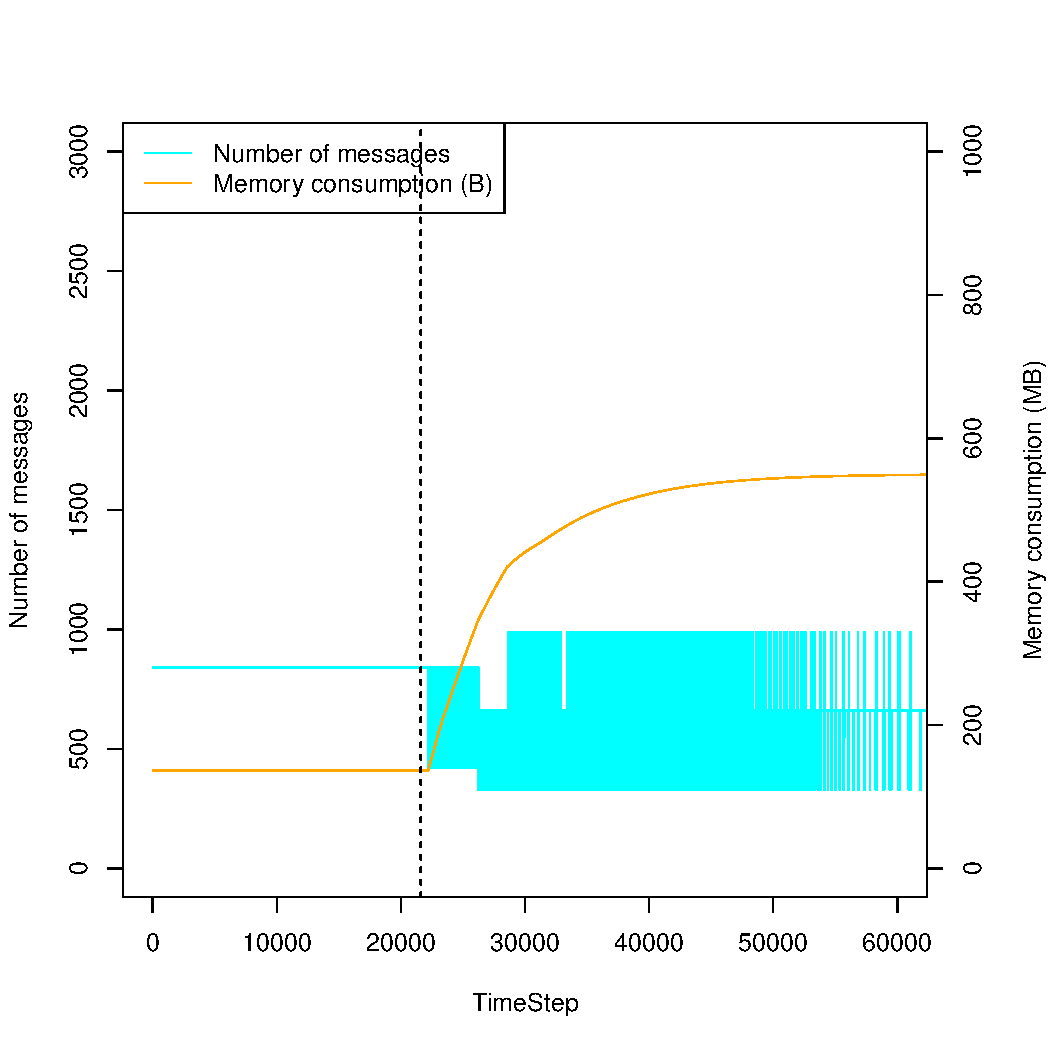
\includegraphics[width=1.0\hsize]{scenario_5_signaling_and_memoryload_vs_timeStep_86400_345600_1_0_0_0_ideal.pdf}
   \subcaption{CPU負荷とメモリ使用量の変化}
   \label{subfig:scenario_5_signaling_and_memoryload_vs_timeStep_86400_345600_1_0_0_0_ideal}
 \end{subfigure}
 \begin{subfigure}{0.49\hsize}
   \centering
   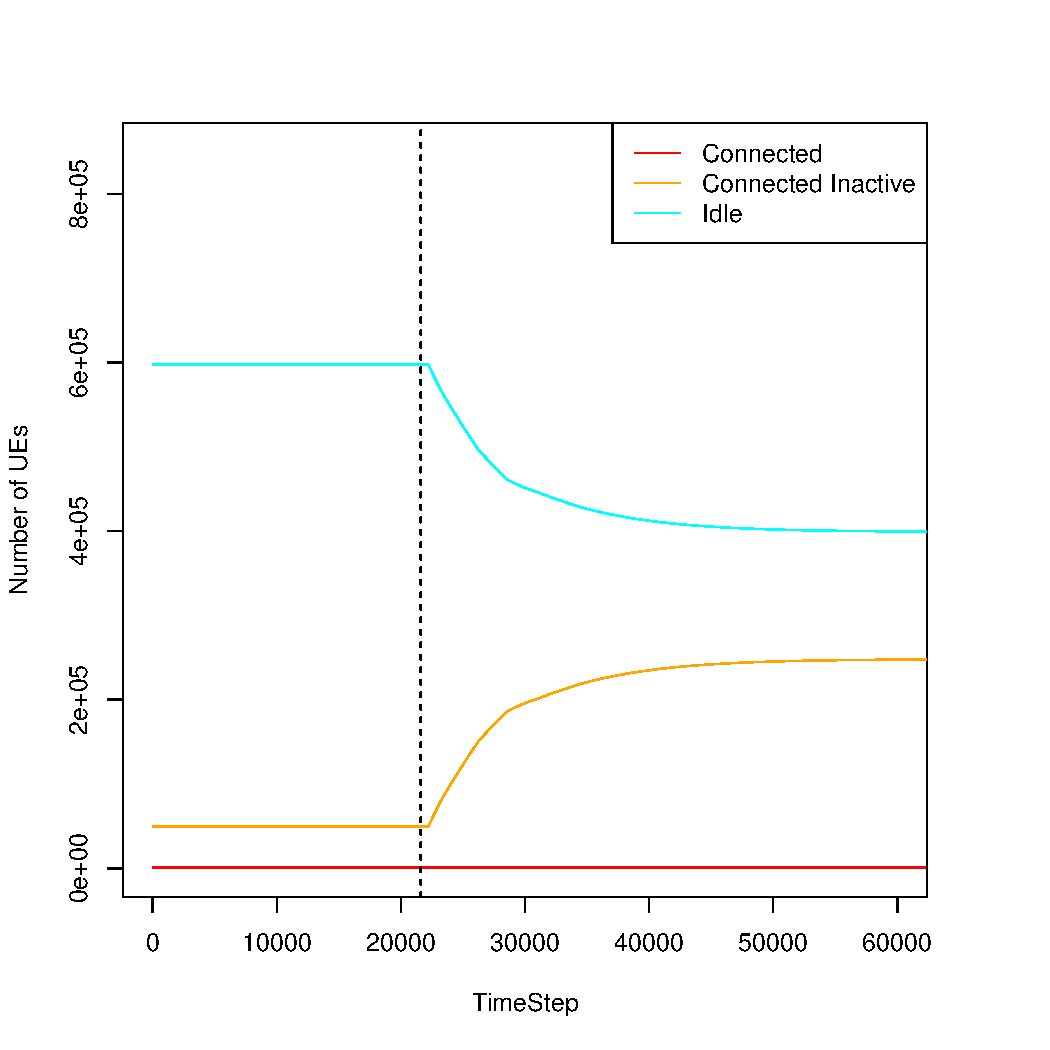
\includegraphics[width=1.0\hsize]{scenario_5_stateBreakdown_86400_345600_1_0_0_0_ideal.pdf}
   \subcaption{各状態にあるUE台数の変化}
   \label{subfig:scenario_5_stateBreakdown_86400_345600_0130900-pideal}
 \end{subfigure}
 \caption{理想PID($K_p = 1、K_i = 0、K_d = 0$)}
 \label{fig:result_pid_ideal_1_0_0_0}

\end{figure}

\begin{figure}[htbp]
 \centering
 \begin{subfigure}{0.49\hsize}
   \centering
   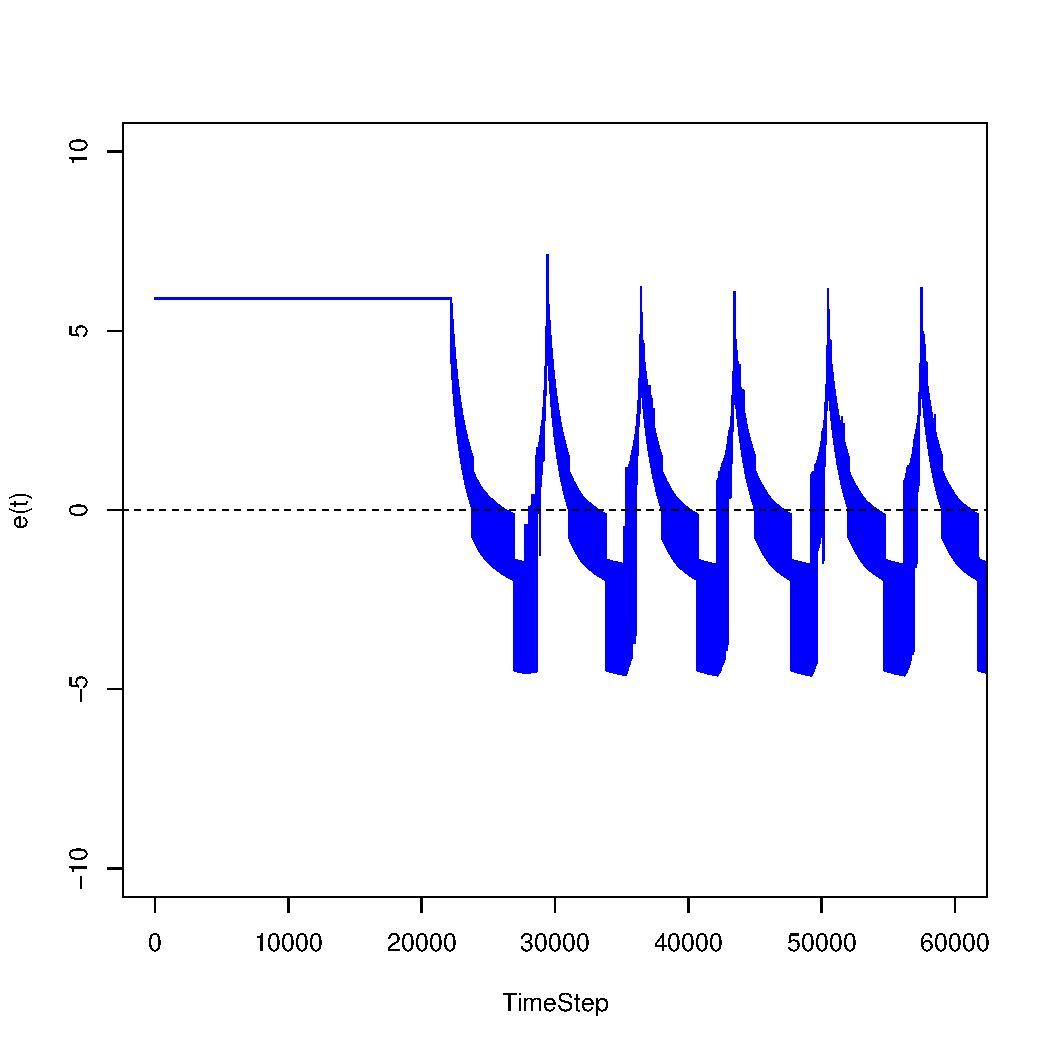
\includegraphics[width=1.0\hsize]{scenario_5_e_86400_345600_5_0_0_0_ideal.pdf}
   \subcaption{$e(t)$の変化}
   \label{subfig:scenario_5_e_86400_345600_0-318_5_0_0_0_ideal}
 \end{subfigure}
 \begin{subfigure}{0.49\hsize}
   \centering
   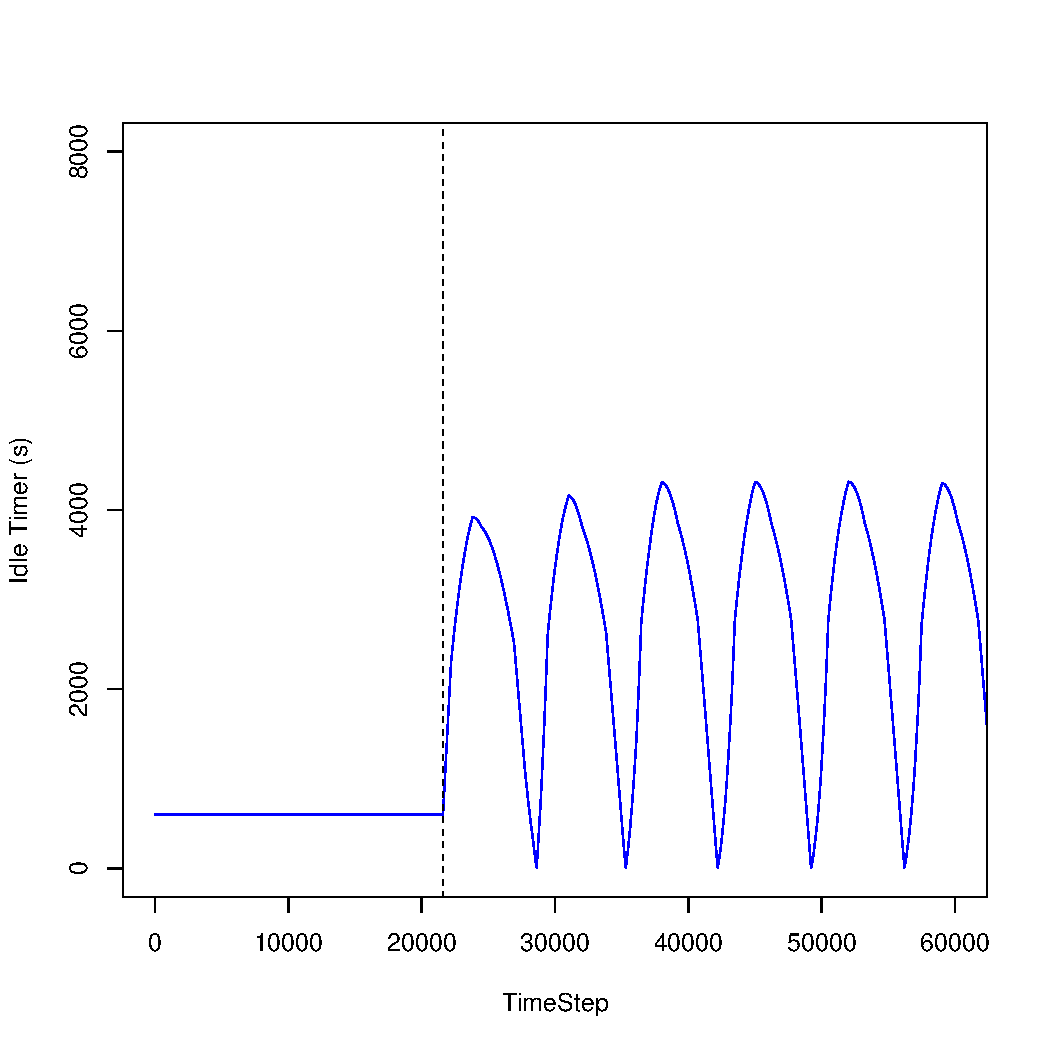
\includegraphics[width=1.0\hsize]{scenario_5_idleTimer_86400_345600_5_0_0_0_ideal.pdf}
   \subcaption{IdleTimerの変化}
   \label{subfig:scenario_5_idleTimer_86400_345600_5_0_0_0_ideal}
 \end{subfigure}
 \par\bigskip %改行
 \begin{subfigure}{0.49\hsize}
   \centering
   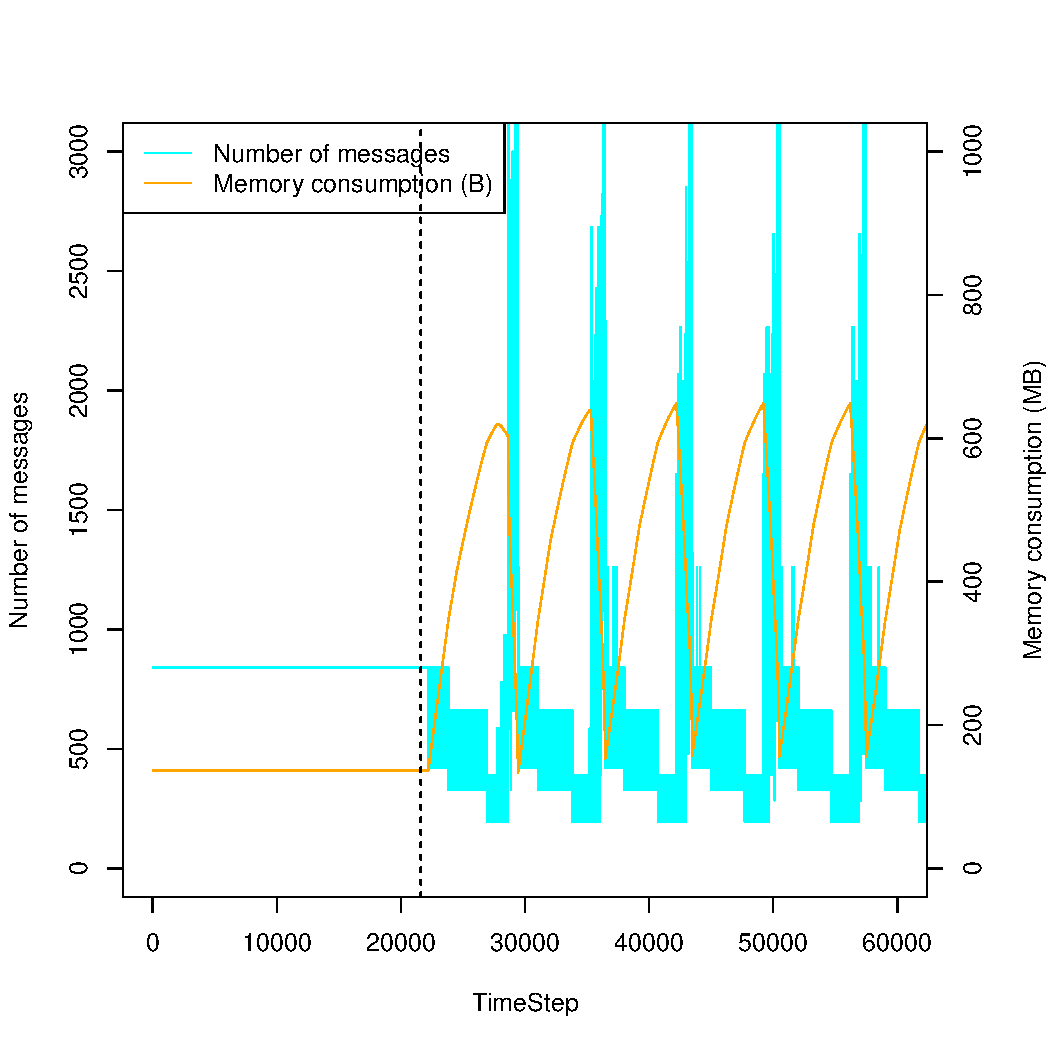
\includegraphics[width=1.0\hsize]{scenario_5_signaling_and_memoryload_vs_timeStep_86400_345600_5_0_0_0_ideal.pdf}
   \subcaption{CPU負荷とメモリ使用量の変化}
   \label{subfig:scenario_5_signaling_and_memoryload_vs_timeStep_86400_345600_5_0_0_0_ideal}
 \end{subfigure}
 \begin{subfigure}{0.49\hsize}
   \centering
   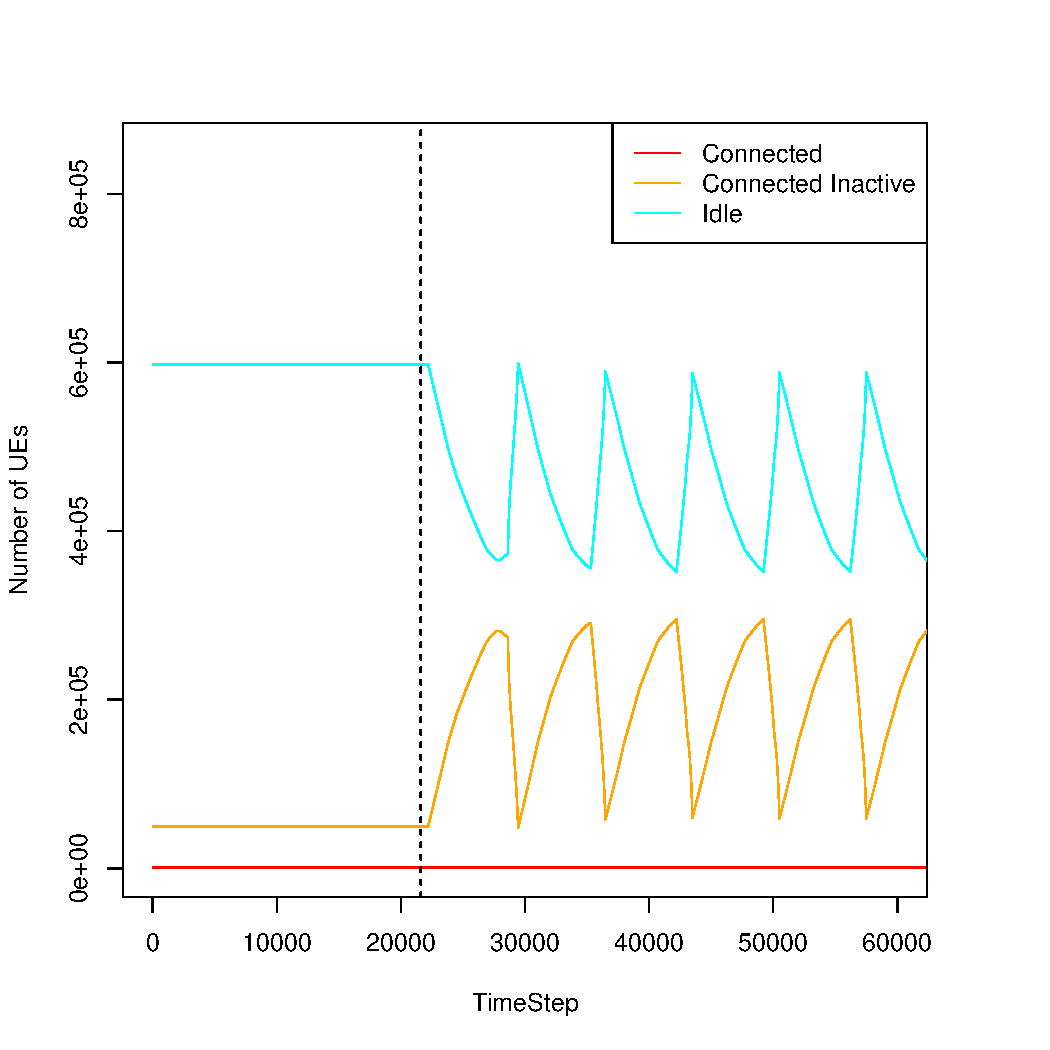
\includegraphics[width=1.0\hsize]{scenario_5_stateBreakdown_86400_345600_5_0_0_0_ideal.pdf}
   \subcaption{各状態にあるUE台数の変化}
   \label{subfig:scenario_5_stateBreakdown_86400_345600_5_0_0_0_ideal}
 \end{subfigure}
 \caption{理想PID($K_p = 5、K_i = 0、K_d = 0$)}
 \label{fig:result_pid_ideal_5_0_0_0}
\end{figure}







\end{document}
